%===============================================================================
% LaTeX sjabloon voor de bachelorproef toegepaste informatica aan HOGENT
% Meer info op https://github.com/HoGentTIN/bachproef-latex-sjabloon
%===============================================================================

\documentclass{bachproef-tin}

\usepackage{hogent-thesis-titlepage} % Titelpagina conform aan HOGENT huisstijl
\usepackage[english]{babel}

%%---------- Documenteigenschappen ---------------------------------------------

% De titel van het rapport/bachelorproef
\title{Best practices om continuous integration en continuous delivery uit te rollen in een SAPUI5 webapplicatie op SAP Cloud Platform}

% Je eigen naam
\author{Renaat Haleydt}

% De naam van je promotor (lector van de opleiding)
\promotor{Harm De Weirdt}

% De naam van je co-promotor. Als je promotor ook je opdrachtgever is en je
% dus ook inhoudelijk begeleidt (en enkel dan!), mag je dit leeg laten.
\copromotor{Pieter-Jan Deraedt}

% Indien je bachelorproef in opdracht van/in samenwerking met een bedrijf of
% externe organisatie geschreven is, geef je hier de naam. Zoniet laat je dit
% zoals het is.
\instelling{Amista}

% Academiejaar
\academiejaar{2018-2019}

% Examenperiode
%  - 1e semester = 1e examenperiode => 1
%  - 2e semester = 2e examenperiode => 2
%  - tweede zit  = 3e examenperiode => 3
\examenperiode{2}

%===============================================================================
% Inhoud document
%===============================================================================

\begin{document}

%---------- Taalselectie -------------------------------------------------------
% Als je je bachelorproef in het Engels schrijft, haal dan onderstaande regel
% uit commentaar. Let op: de tekst op de voorkaft blijft in het Nederlands, en
% dat is ook de bedoeling!

%\selectlanguage{english}

%---------- Titelblad ----------------------------------------------------------
\inserttitlepage

%---------- Samenvatting, voorwoord --------------------------------------------
\usechapterimagefalse
%%=============================================================================
%% Voorwoord
%%=============================================================================

\chapter*{\IfLanguageName{dutch}{Woord vooraf}{Preface}}
\label{ch:voorwoord}

%% TODO:
%% Het voorwoord is het enige deel van de bachelorproef waar je vanuit je
%% eigen standpunt (``ik-vorm'') mag schrijven. Je kan hier bv. motiveren
%% waarom jij het onderwerp wil bespreken.
%% Vergeet ook niet te bedanken wie je geholpen/gesteund/... heeft


%%=============================================================================
%% Samenvatting
%%=============================================================================

% TODO: De "abstract" of samenvatting is een kernachtige (~ 1 blz. voor een
% thesis) synthese van het document.
%
% Deze aspecten moeten zeker aan bod komen:
% - Context: waarom is dit werk belangrijk?
% - Nood: waarom moest dit onderzocht worden?
% - Taak: wat heb je precies gedaan?
% - Object: wat staat in dit document geschreven?
% - Resultaat: wat was het resultaat?
% - Conclusie: wat is/zijn de belangrijkste conclusie(s)?
% - Perspectief: blijven er nog vragen open die in de toekomst nog kunnen
%    onderzocht worden? Wat is een mogelijk vervolg voor jouw onderzoek?
%
% LET OP! Een samenvatting is GEEN voorwoord!

%%---------- Nederlandse samenvatting -----------------------------------------
%
% TODO: Als je je bachelorproef in het Engels schrijft, moet je eerst een
% Nederlandse samenvatting invoegen. Haal daarvoor onderstaande code uit
% commentaar.
% Wie zijn bachelorproef in het Nederlands schrijft, kan dit negeren, de inhoud
% wordt niet in het document ingevoegd.

\IfLanguageName{english}{%
\selectlanguage{dutch}
\chapter*{Samenvatting}
\lipsum[1-4]
\selectlanguage{english}
}{}

%%---------- Samenvatting -----------------------------------------------------
% De samenvatting in de hoofdtaal van het document

\chapter*{\IfLanguageName{dutch}{Samenvatting}{Abstract}}

\lipsum[1-4]


%---------- Inhoudstafel -------------------------------------------------------
\pagestyle{empty} % Geen hoofding
\tableofcontents  % Voeg de inhoudstafel toe
\cleardoublepage  % Zorg dat volgende hoofstuk op een oneven pagina begint
\pagestyle{fancy} % Zet hoofding opnieuw aan

%---------- Lijst figuren, afkortingen, ... ------------------------------------

% Indien gewenst kan je hier een lijst van figuren/tabellen opgeven. Geef in
% dat geval je figuren/tabellen altijd een korte beschrijving:
%
%  \caption[korte beschrijving]{uitgebreide beschrijving}
%
% De korte beschrijving wordt gebruikt voor deze lijst, de uitgebreide staat bij
% de figuur of tabel zelf.

\listoffigures
\listoftables

% Als je een lijst van afkortingen of termen wil toevoegen, dan hoort die
% hier thuis. Gebruik bijvoorbeeld de ``glossaries'' package.
% https://www.overleaf.com/learn/latex/Glossaries

%---------- Kern ---------------------------------------------------------------

% De eerste hoofdstukken van een bachelorproef zijn meestal een inleiding op
% het onderwerp, literatuurstudie en verantwoording methodologie.
% Aarzel niet om een meer beschrijvende titel aan deze hoofstukken te geven of
% om bijvoorbeeld de inleiding en/of stand van zaken over meerdere hoofdstukken
% te verspreiden!

%%=============================================================================
%% Inleiding
%%=============================================================================

\chapter{\IfLanguageName{dutch}{Inleiding}{Introduction}}
\label{ch:inleiding}

De inleiding moet de lezer net genoeg informatie verschaffen om het onderwerp te begrijpen en in te zien waarom de onderzoeksvraag de moeite waard is om te onderzoeken. In de inleiding ga je literatuurverwijzingen beperken, zodat de tekst vlot leesbaar blijft. Je kan de inleiding verder onderverdelen in secties als dit de tekst verduidelijkt. Zaken die aan bod kunnen komen in de inleiding~\autocite{Pollefliet2011}:

\begin{itemize}
  \item context, achtergrond
  \item afbakenen van het onderwerp
  \item verantwoording van het onderwerp, methodologie
  \item probleemstelling
  \item onderzoeksdoelstelling
  \item onderzoeksvraag
  \item \ldots
\end{itemize}

\section{\IfLanguageName{dutch}{Probleemstelling}{Problem Statement}}
\label{sec:probleemstelling}

Uit je probleemstelling moet duidelijk zijn dat je onderzoek een meerwaarde heeft voor een concrete doelgroep. De doelgroep moet goed gedefinieerd en afgelijnd zijn. Doelgroepen als ``bedrijven,'' ``KMO's,'' systeembeheerders, enz.~zijn nog te vaag. Als je een lijstje kan maken van de personen/organisaties die een meerwaarde zullen vinden in deze bachelorproef (dit is eigenlijk je steekproefkader), dan is dat een indicatie dat de doelgroep goed gedefinieerd is. Dit kan een enkel bedrijf zijn of zelfs één persoon (je co-promotor/opdrachtgever).

\section{\IfLanguageName{dutch}{Onderzoeksvraag}{Research question}}
\label{sec:onderzoeksvraag}

Wees zo concreet mogelijk bij het formuleren van je onderzoeksvraag. Een onderzoeksvraag is trouwens iets waar nog niemand op dit moment een antwoord heeft (voor zover je kan nagaan). Het opzoeken van bestaande informatie (bv. ``welke tools bestaan er voor deze toepassing?'') is dus geen onderzoeksvraag. Je kan de onderzoeksvraag verder specifiëren in deelvragen. Bv.~als je onderzoek gaat over performantiemetingen, dan 

\section{\IfLanguageName{dutch}{Onderzoeksdoelstelling}{Research objective}}
\label{sec:onderzoeksdoelstelling}

Wat is het beoogde resultaat van je bachelorproef? Wat zijn de criteria voor succes? Beschrijf die zo concreet mogelijk. Gaat het bv. om een proof-of-concept, een prototype, een verslag met aanbevelingen, een vergelijkende studie, enz.

\section{\IfLanguageName{dutch}{Opzet van deze bachelorproef}{Structure of this bachelor thesis}}
\label{sec:opzet-bachelorproef}

% Het is gebruikelijk aan het einde van de inleiding een overzicht te
% geven van de opbouw van de rest van de tekst. Deze sectie bevat al een aanzet
% die je kan aanvullen/aanpassen in functie van je eigen tekst.

De rest van deze bachelorproef is als volgt opgebouwd:

In Hoofdstuk~\ref{ch:stand-van-zaken} wordt een overzicht gegeven van de stand van zaken binnen het onderzoeksdomein, op basis van een literatuurstudie.

In Hoofdstuk~\ref{ch:methodologie} wordt de methodologie toegelicht en worden de gebruikte onderzoekstechnieken besproken om een antwoord te kunnen formuleren op de onderzoeksvragen.

% TODO: Vul hier aan voor je eigen hoofstukken, één of twee zinnen per hoofdstuk

In Hoofdstuk~\ref{ch:conclusie}, tenslotte, wordt de conclusie gegeven en een antwoord geformuleerd op de onderzoeksvragen. Daarbij wordt ook een aanzet gegeven voor toekomstig onderzoek binnen dit domein.
\chapter{\IfLanguageName{dutch}{Continuous Integration, Continuous Delivery \& Continuous Deployment}{Continuous Integration, Continuous Delivery \& Continuous Deployment}}
\label{ch:ci-cd-cd}
    \section{Algemeen}
    \label{sec:algemeen}
    Bedrijven zijn constant op zoek naar betere en snellere resultaten. In het software development circuit is het vandaag soms nog lang wachten voor een wijziging effectief doorgevoerd wordt. Men levert nog vaak software op aan het einde van de sprint, wat soms voor problemen zorgt als men veel code tegelijk aflevert. Met een nieuwe software development methode - Continuous Integration en Continuous Delivery genaamd - wil men deze problemen zoveel mogelijk vermijden. Er wordt vaak gesproken van een CI/CD pipeline als het gaat over Continuous Integration en Continuous Delivery, maar er is nog een derde speler dat men kan invoeren: Continuous Deployment. Samen vormen zij de 3 musketiers om software projecten een grotere slaagkans te geven.
    Om een duidelijker beeld te scheppen van een CI/CD pipeline zal dit hoofdstuk eerst uitleg verschaffen over DevOps, omdat dit de allesomvattende term is waar de 3 musketiers deel van uitmaken. Er wordt ook dieper ingegaan op Continuous Integration, Continuous Delivery, Continuous Deployment en tot slot komt Automated Testing aan bod.
        \paragraph{DevOps}
        DevOps is een samentrekking van development en operations en is een welbekend begrip binnen de informatica wereld. Het heeft als doel om de 'state of mind' binnen een bedrijf te veranderen zodat alle lagen/departementen vlotter samenwerken. Het is een praktische 'gids' dat bedrijven kunnen gebruiken om de communicatie tussen developers en systeembeheerders beter te maken. Deze twee verschillende lagen in een bedrijf willen namelijk hetzelfde: zo snel mogelijk kwaliteitsvolle software opleveren. DevOps is gebaseerd op Agile development, maar gaat verder dan dat. Het gaat dieper in op automatisatie, integratie, samenwerking en communicatie. 
        Continuous Integration, Delivery en Deployment zijn kenmerkend voor DevOps, omdat het mee inzet op snellere oplevering van kwaliteitsvolle software. ~\autocite{Riti2018}
        
        %TODO: Hier zeker Patrick Debois vernoemen en vermelden waarom DevOps is opgericht: omdat ze in 2008 veel te maken hadden met falende projecten vanwege slechte communicatie.
    
        \paragraph{Continuous Integration}
        Dit is een eerste stap in de pipeline waarbij de geschreven code wordt gecommit naar een 'repository management server'. Hierdoor wordt de 'source code' automatisch opnieuw opgebouwd en slaagt voor de testen die automatisch zijn opgestart. De focus bij deze stap ligt bij de teamleden ~\autocite{Fowler2006}, van hen wordt verwacht dat ze - op regelmatige basis - hun code pushen (integreren met de master applicatie). Een goede samenwerking tussen de verschillende leden van het development team is broodnodig om tot het gewenste eindresultaat te komen.
        Het doel van een Continuous Integration is om de integratie feilloos te laten verlopen wanneer men software ontwikkelt en geen functionaliteiten verliezen na een merge ~\autocite{Riti2018}.
        
        Bovenstaande uitleg is makkelijker te begrijpen aan de hand van een voorbeeld. Op Figuur \ref{img-ci-example} is een grafische voorstelling van dit voorbeeld terug te vinden.
        De developer maakt een wijziging en commit de code naar de repository die te vinden is op het source-control systeem. De Continuous Integration server krijgt het bericht dat er code is toegevoegd, haalt de laatst toegevoegde code op en laat de testen runnen. Wanneer alle testen slagen zal de CI server de code compilen en feedback bezorgen aan de developer. In dit voorbeeld is er gebruik gemaakt van een externe mail server om die feedback te verzenden.
        Deze stappen gebeuren elke keer er code naar de repository gestuurd wordt.
        Bovenstaand voorbeeld is een best-practice hoe het zou moeten gebeuren. Er zijn echter enkele zaken die wat extra uitleg kunnen gebruiken.
        De frequentie en hoeveelheid code zijn belangrijke zaken waar de developer rekening mee moet houden bij een CI pipeline. Volgens \textcite{Fowler2006} is het de plicht van een developer om minstens 1 maal per dag een commit te doen. Hij moet telkens een commit uitvoeren wanneer hij een kleine opdracht afgerond heeft. Zo blijft de hoeveelheid code klein en is het makkelijk om te zoeken wanneer er zich een probleem voordoet.
        Eens de wijziging gecommit is naar de version control repository moet de CI pipeline zijn werk doen. Een belangrijke stap is het bezorgen van de feedback. Dit moet namelijk het resultaat van de build en de feedback waar het probleem zich kan bevinden terug geven, door bijvoorbeeld aan te geven welke test niet slaagt bij het uitvoeren van de automated testing. De key factor hier is de tijd. Als de developer pas daags nadien feedback krijgt over de fout die hij gepusht heeft, wordt het al moeilijker om de fout te vinden en ze op te lossen. 
        \begin{figure}	
            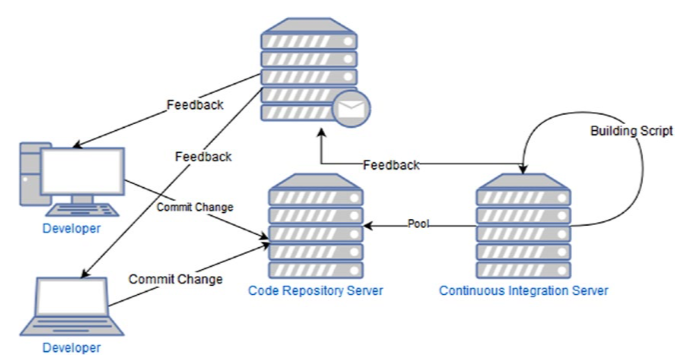
\includegraphics[scale=0.65]{ci-example}
            \caption{Voorbeeld van een Continuous Integration set-up ~\autocite{Riti2018}} \label{img-ci-example}
        \end{figure}
    
        \paragraph{Continuous Delivery}
        Eens het team met succes de Continuous Integration toepast kan men overschakelen naar de volgende stap: Continuous Delivery.
        Het is een manier dat ervoor zorgt dat de code die van de Continuous Integration stap komt, gebuild en voorbereid wordt voor een release.
        Er is echter wel nog een menselijke hand nodig om de build van deze stap te deployen en voor de buitenwereld beschikbaar te stellen ~\autocite{Fowler2013}.
        \newline{}In Figuur \ref{img-cd-chain} wordt de opbouw van een Continuous Delivery chain weergegeven, het is een grafische weergave van de stappen die een Continuous Delivery pipeline moet hebben. Dit is gebaseerd op de Continuous Integration chain, maar hier zijn extra stappen toegevoegd.
        De eerste stap is het developen van de code die men wenst op te leveren. Net zoals bij Continuous Integration commit de developer de code naar de version control repository. De build scheduler haalt de laatst toegevoegde code op en test deze code. Enkel bij het slagen van alle testen wordt de code gebuild door de build scheduler. Deze maakt ook de build klaar voor release en vereist enkel nog menselijke goedkeuring om deze release te lanceren.
        \newline{}In dit proces is feedback ook uiterst belangrijk. Wanneer developers foute code pushen, moet de persoon die de foute code geschreven heeft zo snel mogelijk verwittigd worden. Op deze manier kan het euvel snel opgelost worden.
        Mail kan een vorm zijn van feedback, maar er bestaan nog andere leuke vormen naast mailing. Het bedrijf Dynatrace heeft bijvoorbeeld een licht ontworpen dat je in de kamer van het team kan hangen. Dit Internet of Things (IoT) gadget, DevOps UFO genaamd, is via WiFi verbonden aan de pipeline omgeving. Het geeft feedback over de staat van de CI/CD pipeline en is een vorm van monitoring. Het geeft de developers en iedereen in de kamer onmiddelijke feedback wanneer er een commit gebeurd. Als de commit door de pipeline geraakt zal de UFO groen kleuren, wanneer de build faalt kleurt de UFO rood en weet iedereen dat er een fout is. Zo weet de persoon die de foute code gepusht heeft dat er iets fout is en kan hij hier nog sneller op inspelen. 
        \begin{figure}	
            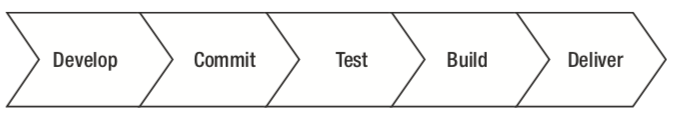
\includegraphics[scale=0.65]{cd-chain}
            \caption{Continuous Delivery chain ~\autocite{Riti2018}} \label{img-cd-chain}
        \end{figure}
        
        \paragraph{Continuous Deployment}
        De gelijkenis met Continuous Deployment is treffend, maar er is wel degelijk een verschil.
        Hier gaat men automatisch de veranderde code naar productie brengen. De veranderingen gaan door de volledige pipeline en eens ze slagen voor alle testen wordt - zonder menselijke interactie - de code naar productie gebracht ~\autocite{Claps2015}.
        Dit wordt soms ook wel de 'train to production' genoemd, omdat elke code dat gepusht wordt naar de source-control automatisch tot bij de klant geraakt.
        
        \paragraph{Automated Testing}
        Zoals hierboven reeds aangegeven is er geen Continuous Integration pipeline zonder automated testing. Het grootste doel van deze fase is - zoals de naam het zegt - testen van de code. Als de CI/CD pipeline voorzien wordt van voldoende en goede testen, wordt er een veiligheidsgevoel gecreëerd. Op deze manier voldoet de software aan bepaalde criteria, die in de testen verwerkt worden. Het is dus een heel belangrijk onderdeel van de pipeline waar veel aandacht aan besteed moet worden. 
        Om te voldoen aan de criteria van CI/CD moeten de testen automatisch gerund worden. Dit was tot voor kort echter vaak niet het geval. Er waren testers aangesteld om telkens opnieuw software te testen, door op de verschillende knoppen te drukken in de user interface (UI). Heel vaak slopen er fouten in omdat dit heel repetitief en saai werk was. Daar komt de automatisatie van pas ~\autocite{Vocke2018}.
        
        Mike Cohn kwam met het idee om testen op te delen in drie grote categorieën: Unit Tests, Service Tests en UI tests zoals u kan zien in Figuur \ref{img-test-pyramid}.
        Vandaag zijn deze categorieën iets te simplistisch voorgesteld, vanwege de toenemende complexiteit van de software. Maar het is wel nog altijd een uitstekende referentie om de opbouw van testen uit te leggen.
        Twee zaken zijn belangrijk om te onthouden: testen moeten uit verschillende lagen van detail bestaan en er moeten minder testen geschreven worden wanneer het team minder gedetailleerd (high-level testing) gaat. Omdat bij high-level testen de requirements goed begrepen zijn door het test team.
        De grootste laag binnen de test omgeving zijn de Unit tests en staat het dichts bij de software code. Deze testen zijn snel om te schrijven en te runnen en kunnen gedetailleerde feedback geven wanneer een test faalt.
        De laag erboven service tests - ook wel Integration tests genoemd - focust vooral op de functionaliteit van de applicatie.
        Deze testen leggen de nadruk op de functionaliteit dat de applicatie moet bevatten. Ze testen de API calls en de integratie van de individuele functies.
        De kleinste laag zijn de UI tests, ook wel end-to-end testen genoemd. Deze testen de user interface door bijvoorbeeld op knoppen te drukken, formulieren in te vullen of te navigeren doorheen de applicatie. Het nadeel van deze testen zijn dat ze fragiel, duur en tijdrovend zijn om te bouwen en traag om te runnen zijn.
        Om de snelheid te garanderen en de hoeveelheid build times klein te houden is het belangrijk de vorm van de piramide te behouden. Het gevaar dreigt om de test omgeving als een ijsjes hoorn te vormen met meer UI tests dan Unit tests ~\autocite{Fowler2012}.
        \begin{figure}	
            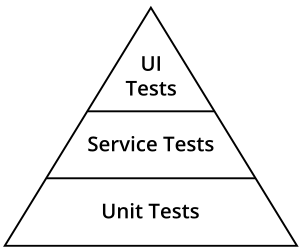
\includegraphics[scale=0.65]{test-pyramid}
            \caption{Test piramide ~\autocite{Vocke2018}} \label{img-test-pyramid}
        \end{figure}
    
    %TODO: nog nakijken van onderstaande tekst. Hier moeten de lagen van de CI/CD pipeline besproken worden en hun tools kort aangehaald worden.
    \section{Lagen binnen een CI/CD pipeline en beschikbare tools}
    \label{sec:lagen-binnen-pipeline}
    Er bestaan verschillende repository management services die een source control systeem hebben. GitHub, GitLab en Bitbucket zijn enkele voorbeelden.
    Build schedulers zorgen ervoor dat de procedures worden samengesteld en dat de builds worden getriggerd. Voorbeelden hiervan zijn: Jenkins, Travis CI, GitLab-CI en Bamboo. Sonatype Nexus en Archiva zijn dan weer voorbeelden van tools die gebruikt worden als artifact repository manager, deze houden bij wijze van spreken de code bij die klaar is om te deployen. 
    
        \paragraph{Source Control System}
        Dit systeem houdt alle veranderingen bij aan de code en zal de veranderingen ook beheren zodat ze niet overlappen. Het laat toe dat meerdere developers tegelijk aan - soms dezelfde - code werken. Een source control systeem houdt dan de veranderingen bij wat elke developer gedaan heeft. Best practice is er maar 1 versie van de software die stabiel is, meestal master genoemd. Een gangbare praktijk binnen dit systeem is het maken van branches. Hier wordt een kopie gemaakt van de stabiele master, waardoor men wat kan knoeien in de branch zonder de master te beschadigen. Als men overtuigd is van de kwaliteiten dat men op een branch gemaakt heeft kan men de branch 'mergen' in de master. Deze techniek wordt ook wel 'revision control' of 'version control' genoemd ~\autocite{Skelton2014} en ~\autocite{Riti2018}.
        Voorbeelden van zo een source control system zijn Git, CVS (Concurrent Version System), Subversion en Mercurial.
        
        \paragraph{Repository Management Services}
        Wordt ook wel Code Repository Server genoemd. Hier wordt de software van het source control system opgeslagen. Dit kan op een interne server opgeslagen worden, of op een externe die door bedrijven aangeboden wordt. Dit maakt het makkelijker voor developers om samen te werken en dezelfde bron te gebruiken en is nodig om een goede Continuous Integration aan te bieden.
    
        \paragraph{Build Scheduler}
        Een Build Scheduler kan ook wel een Continuous Integration Server genoemd worden.
        Dit zorgt ervoor dat - telkens wanneer er code gecommit wordt - de pipeline wordt uitgevoerd. De taken van de build scheduler zijn: 
        \begin{itemize}
            \item Code ophalen van de Repository Server en deze samenvoegen met de oude code
            \item De testen uitvoeren
            \item Het builden van de software
            \item Feedback geven aan de developer over voorgaande stappen
        \end{itemize}
        Deze taken kunnen ook door een script volbracht worden, maar het is belangrijk dat deze taken automatisch gebeuren telkens er code gecommit wordt naar de repository manager ~\autocite{Riti2018}.
        
        \paragraph{Artifact Repository Manager}
        Als laatste zijn de Artifact Repository Managers aan de beurt. Deze repository manager houdt alles wat nodig is om de applicatie te deployen bij zoals
        \begin{itemize}
            \item packaged application code
            \item application assets
            \item infrastructure code
            \item virtual machine images
            \item configuration data
        \end{itemize}
        Deze tool houdt alle geschiedenis bij van de bovenstaande files. Zoals eerder vermeld kan men vanaf hier de software (automatisch) deployen. Dit is de allerlaatste fase in de CI/CD pipeline ~\autocite{Skelton2014}.
%%=============================================================================
%% Onderzoeksdomein1
%%=============================================================================

\chapter{\IfLanguageName{dutch}{Voor- en nadelen CI/CD pipeline}{Research field 1: benefits and drawbacks of a CI/CD pipeline}}
\label{ch:voor-en-nadelen-cicd}
Dit gaat over de algemene voordelen van zo een pipeline, maar ook specifiek van Amista. Om een antwoord te krijgen op de algemene voordelen wordt er als basis teruggegrepen naar de literatuur. Er is namelijk al enorm veel geschreven over een CI/CD pipeline en wat de voor- en nadelen kunnen zijn.
Bijkomstig is er een interview afgenomen met de expert omtrent DevOps, Patrick Debois.
Het interview en de literatuur bieden samen de perfecte combinatie om de voordelen en nadelen te bespreken.
Op de vraag wat de voor- en nadelen voor Amista zullen zijn kan enkel iemand van Amista op antwoorden natuurlijk. Er zijn vragen gesteld aan Pieter-Jan Deraedt om te kijken hoe Amista denkt te winnen bij het integreren van een CI/CD pipeline.


\section{Voordelen}
\label{sec:voordelen}
\begin{itemize}
    \item Als men kleine stukjes code commit naar de centrale repository en de testen slagen niet, weet men dat het aan dit klein deeltje van de code ligt en kan men de fout veel sneller opsporen.
    \item In de meeste omgevingen met een CI/CD pipeline is het niet nodig om een QA team te hebben om de testen uit te voeren, wat de kosten doet dalen natuurlijk.
\end{itemize}

\section{Nadelen}
\label{sec:nadelen}

\chapter{\IfLanguageName{dutch}{SAP}{SAP}}
\label{ch:sap}
SAP is een Duitse onderneming opgericht in 1972 dat softwareoplossingen aanbiedt voor grote ondernemingen. Met meer dan 413.000 klanten verspreid over 180 landen mag SAP zich marktleider noemen op gebied van bedrijfssoftware.
SAP heeft zicht gespecialiseerd in ERP, Enterprise Resource Planning software dat alle processen van het bedrijf automatiseert ~\autocite{SAPERP2019}. Een ERP systeem beheert meerdere functies en bedrijfsprocessen van één bedrijf op basis van een centrale database. Het heeft als doel de gegevens van de organisatie optimaal te gebruiken in de gehele organisatie en een betere beheersing van de bedrijfsprocessen voorzien.
De oplossingen die SAP aanbiedt zijn vooral bedoeld voor de grotere bedrijven. Ze bieden software aan voor elke mogelijke industrie die er vandaag de dag bestaat, maar pakken uit met hun specialiteiten in de cloud business software.
Hieronder worden kort de programma's beschreven die gebruikt worden in de voorbeeldapplicatie. Het geeft een grof beeld van de omgeving waar Amista graag een CI/CD pipeline wil voor integreren.

    \paragraph{SAP Cloud Platform}
    SAP Cloud Platform is een platform as a service (PaaS), dat aangeboden wordt door SAP. het is een online platform dat - door hardware en software samen te brengen - applicaties overal toegankelijk maakt en samenbrengt tot één platform online ~\autocite{SAPSE2018}.
    SAP Cloud Platform wordt zowel voor development als deployment gebruikt, maar reikt ook de hand aan verschillende technologieën: Internet of Things, Big Data, Artificiële Intelligentie enzovoort. Het is een platform dat zowel on-premise - waarbij software enkel lokaal op een computer beschikbaar is - als cloud technologieën samen kan brengen. Je kan er de technologieën ook uitbreiden en zelf ontwikkelen. Het haalt zijn kracht uit de perfecte integratie met andere SAP software die je ook nog eens kan uitbreiden.
    
    \paragraph{SAPUI5}
    SAPUI5 is een framework dat uitgevonden is door SAP en bevat verschillende libraries die bovenop JavaScript gebouwd zijn. Via het SAP Cloud Platform kunnen er front-end applicaties gemaapkt en deployed worden die geschreven zijn in SAPUI5. Het is een framework dat bedoeld is om HTML5 applicaties te bouwen die bijna automatisch responsive zijn zonder veel bijkomende code toe te voegen.
    Het is bedoeld om dezelfde lay-out en hetzelfde gebruik voor de eindklant te garanderen. Het biedt aan de developers een resem aan UI controls aan, zodat er een consistenter en beter UX design gehanteerd wordt.~\autocite{SAPSEa} 
    
    \paragraph{SAP HANA}
    In-Memory Data Platform staat als titel op de site van SAP te lezen. Het is een platform dat gebruik maakt van het RAM-geheugen van de computer, wat enorme snelheden met zich meebrengt, maar ook een enorm kostenplaatje. Dit even terzijde wordt SAP Hana aangeprezen als een platform om ingewikkelde, real-time analytische berekeningen uit te voeren op data.
    Het is een Relationeel Database Management Systeem (RDMBMS) dat geïntegreerd kan worden in SAP Cloud Platform, waarbij het mogelijk is om zowel on-premise als in de cloud te werken, of een combinatie van beiden.

%%=============================================================================
%% Methodologie
%%=============================================================================

\chapter{\IfLanguageName{dutch}{Methodologie}{Methodology}}
\label{ch:methodologie}

%% TODO: Hoe ben je te werk gegaan? Verdeel je onderzoek in grote fasen, en
%% licht in elke fase toe welke stappen je gevolgd hebt. Verantwoord waarom je
%% op deze manier te werk gegaan bent. Je moet kunnen aantonen dat je de best
%% mogelijke manier toegepast hebt om een antwoord te vinden op de
%% onderzoeksvraag.

\section{Onderzoeksdomein 1: Wat zijn de voor- en nadelen van een CI/CD pipeline}
\label{sec:onderzoeksdeel1}
Dit gaat over de algemene voordelen van zo een pipeline, maar ook specifiek van Amista. Om een antwoord te krijgen op de algemene voordelen wordt er als basis teruggegrepen naar de literatuur. Er is namelijk al enorm veel geschreven over een CI/CD pipeline en wat de voor- en nadelen kunnen zijn.
Bijkomstig is er een interview afgenomen met de expert omtrent DevOps, Patrick Debois.
Het interview en de literatuur bieden samen de perfecte combinatie om de voordelen en nadelen te bespreken.
Op de vraag wat de voor- en nadelen voor Amista zullen zijn kan enkel iemand van Amista op antwoorden natuurlijk. Er zijn vragen gesteld aan Pieter-Jan Deraedt om te kijken hoe Amista denkt te winnen bij het integreren van een CI/CD pipeline.

\section{Onderzoeksdomein 2: Vergelijken van de beschikbare tools}
\label{sec:onderzoeksdeel2}
Wat zijn voor Amista nu de beste tools om een CI/CD pipeline te integreren in hun software development? Welke tools scoren het beste op vlak van snelheid, configureerbaarheid met SAP en de tools die Amista gebruikt, documentatie die te vinden is online en de kostprijs. 

\section{Onderzoeksdomein 3: Voorbeeldapplicatie dat Amista zal gebruiken}
\label{sec:onderzoeksdeel3}
Hoe ziet de omgeving er uit waar een CI/CD pipeline geïntegreerd moet worden er uit? In de literatuurstudie is de uitleg over de tools terug te vinden, maar hier worden de onderliggende relaties tussen de tools besproken.
Er zal een test omgeving opgezet worden die hier besproken zal worden. 

\section{Onderzoeksdomein 4: Handleiding van een CI/CD pipeline voor een SAPUI5 applicatie op SAP Cloud Platform}
\label{sec:onderzoeksdeel4}
Het eigenlijke doel van deze studie is het maken van een mooie 'handleiding' over de best practices om een CI/CD pipeline op te starten met de winnende tools uit Onderzoeksdomein 2. Zo heeft Amista een 'gepersonaliseerde tutorial' hoe een pipeline op te zetten met de tools die het beste matchen met de noden van het bedrijf zelf.



% \lipsum[21-25]



% Voeg hier je eigen hoofdstukken toe die de ``corpus'' van je bachelorproef
% vormen. De structuur en titels hangen af van je eigen onderzoek. Je kan bv.
% elke fase in je onderzoek in een apart hoofdstuk bespreken.

%%=============================================================================
%% Technische vergelijking tussen build schedulers
%%=============================================================================

\chapter{\IfLanguageName{dutch}{Vergelijking tussen build schedulers}{Comparing build schedulers}}
\label{ch:vergelijking-build-schedulers}

%%=============================================================================
%% Voorbeeldapplicatie
%%=============================================================================

\chapter{\IfLanguageName{dutch}{Voorbeeldapplicatie}{Example of an application}}
\label{ch:voorbeeldapplicatie}
Amista heeft een Ubuntu server ter beschikking gesteld dat wordt gehost op Digital Ocean. De server wordt gebruikt om de build schedulers op te draaien en zo te vergelijken. Eerst moeten er enkele belangrijke zaken ingesteld worden alvorens aan de slag te gaan, zoals security en dergelijke.

    \paragraph{Digital Ocean}
    %TODO: uitleggen wat Digital Ocean is en doet.
    
    \paragraph{Ubuntu server}
    %TODO: Uitleggen welke kenmerken de Ubuntu server heeft.
    
    \paragraph{Installatie Ubuntu server}
    Eerst maken we de Ubuntu server klaar voor gebruik om zo de nodige zaken te installeren.
    %TODO: In figuur EersteKeerInloggenOpUbuntuServer in de bijlagen wordt er getoond wat er moet gebeuren als er voor de eerste keer ingelogd wordt op de server.
    Via de root account wordt er via SSH ingelogd op de server. 
    
    SSH staat voor secure shell en is een software protocol dat voor een veilige verbinding (tunnel) zorgt tussen de client en de server. Het wordt gebruikt voor het configureren van een server, het beheren van netwerken en operating systems. Alle gegevens dat tussen beiden worden uitgevoerd zijn geëncrypteerd waardoor het moeilijker wordt voor hackers om de data te bemachtigen.
    
    Een server die gebruik maakt van SSH wordt ook wel een sshd server genoemd. Eens ingelogd op de sshd server moeten er enkele zaken aangepast worden aan de ssh configuratie in de file /etc/ssh/sshd\_config. Omdat we hier via de root gebruiker werken moet de property PermitRootLogin op yes staan. Dit zorgt ervoor dat de root gebruiker kan inloggen.
    StrictMode moet ook op yes staan, zo kan er niemand inloggen als de authenticatie documenten leesbaar zijn voor iedereen. Dit voor het beveiligen van configuratie documenten. %TODO: Deze configuratie kan u zien in figuur Changing-sshd_config in de bijlagen.
    
    De default manier om in te loggen via ssh is via een account en een paswoord, maar het is ook mogelijk om het account en het paswoord te vervangen door een private en een public key. Dit principe noemt key-based authentication en wordt vooral tijdens development en in scripts gebruikt of voor single sign-on. SSH genereert een private en een public key op de client wanneer deze stap wordt geconfigureerd. De private key moet veilig bewaard worden op de client computer. De public key moet doorgegeven worden aan de remote server. Wanneer de client wil inloggen op de server voert hij een request uit. De server maakt via zijn public key een bericht en stuurt dit als response door naar de client. De client leest het bericht aan de hand van zijn private key en stuurt dan een aangepaste response terug naar de remote server. De server valideert deze response. Bij een geldige private key zal er een goede response verstuurd worden, bij een ongeldige private key een foute response.
    In deze thesis gaat men ervan uit dat de client computer een ssh key heeft die gebruikt kan worden. %TODO: Zoals u in figuur SSHPrivateKeyOnClient kan zien heeft de client die gebruikt werd tijdens het schrijven van deze thesis enkel lees- en schrijfrechten voor de file id\_rsa, dit om het als secret te bewaren.
    De id\_rsa.pub is de publieke key van de client die op de server moet komen om zo de ssh validatie te voorzien, dit wordt ook wel een ssh session genoemd. Eens de ssh session geconfigureerd is zal het niet nodig zijn om via een paswoord in te loggen op de remote server via deze client.
    %TODO: In figuur CopyPublicKeyToServer in de bijlagen is te zien hoe de ssh session wordt opgezet tussen de client en de remote server voor de root user.
    Voor deze thesis en om veiligheidsredenen is het beter om enkel via key-based authenticatie in te loggen en het paswoord uit te sluiten.
    %TODO: In figuur sshd_configNoPassword is te zien welke aanpassingen in de sshd\_config file van de sshd server moeten gebeuren om het niet meer mogelijk te maken om in te loggen via een paswoord. PasswordAuthentication en ChallengeResponseAuthentication moeten naar no verandert worden. PubKeyAuthentication moet naar yes verandert worden.
    Nu moet de sshd\_config file opgeslagen worden (\^x + y + enter) en de ssh daemon herstart worden door het commando sudo systemctl restart ssh in te geven.
    
    Om de remote server nog meer te beschermen tegen cyber aanvallen is het nodig om een firewall op te zetten. In deze voorbeeldapplicatie maken we gebruik van de UFW Firewall. Dis staat voor Uncomplicated Firewall en is een gebruiksvriendelijke tool dat helpt om de iptables onder controle te houden om zo te zorgen dat bepaalde services toegelaten worden tot onze server.
    In Linux maken ze gebruik van het protocol SSH via de service OpenSSH, deze heeft ook een profiel bij UFW.
    %TODO: In Figuur UFWFirewallSetup in de bijlagen is te zien hoe de firewall de SSH service toelaat. Het is enkel mogelijk om de server te bereiken via deze service. Later worden er uiteraard meerdere services toegelaten.
    
    
    
    
    
    
%%=============================================================================
%% Proof-of-concept van een CI/CD pipeline
%%=============================================================================

\chapter{\IfLanguageName{dutch}{Proof-of-concept van een CI/CD pipeline}{Setting up a CI/CD pipeline}}
\label{ch:proof-of-concept}
Uit vorig hoofdstuk is gebleken dat (SCHRAPPEN WAT NIET PAST): Jenkins \& Travis \& Bamboo de tools zijn die aan het meeste must-haves, should-haves en nice-to-haves voldoen. In dit hoofdstuk worden deze tools extra onder de loep genomen door ze op te stellen in een realistische omgeving zoals in hoofdstuk/ref{ch:voorbeeldapplicatie} besproken is. Door de tools te vergelijken in zo'n omgeving krijgen we een meer realistisch beeld welke build-scheduler het beste zal functioneren in deze omgeving. Op het einde van dit hoofdstuk zal er een conclusie worden gemaakt welke build-scheduler Amista moet kiezen en waarom. Maar beginnen doen we met enkele tips te geven van SAP hoe een CI/CD pipeline opgestart moet worden.

\section{Continuous Delivery principles}
\label{sec:continuous-delivery-principles}
Volgens \textcite{Riti2018} is het uitermate belangrijk om volgende stappen te volbrengen om tot een goede Continuous Delivery omgeving te komen.
\begin{itemize}
    \item Er moeten goede branching strategieën bepaald worden om het team goed te laten samenwerken
    \item Een belangrijk onderdeel van Continuous Integration is natuurlijk testen, deze zijn in Continuous Delivery niet te vergeten
    \item Een stap verder is het automatisch uitvoeren van deze testen
    \item Na het slagen van de testen en het automatisch builden van de software moet de build klaar gemaakt worden voor release
\end{itemize}

\section{CI/CD pipeline op SAP Cloud Platform}
\label{sec:ci-cd-op-sap-cloud-platform}
SAP Cloud Platform biedt de mogelijkheid om verschillende omgevingen op te stellen waarin je kan werken als developer. Het vergt enige vereisten om te voldoen aan de regels van Continuous Integration ~\autocite{Kramer2018}:
\begin{itemize}
    \item Hou alles goed bij via een version control systeem
    \item Automatiseer de build
    \item Zorg ervoor dat tijdens de build er Unit testen lopen
    \item Het team moet op regelmatige basis commits uitvoeren
    \item Elke verandering moet gebuild worden
    \item Als er errors tevoorschijn komen tijdens de build, moeten die opgelost worden
    \item De build moet uitgetest worden op een kopie van de productieomgeving
    \item Automatiseer de deployment
\end{itemize}
Eens deze regels zijn toegepast, kunnen we spreken van een CI implementatie.
Vaak wordt CI in combinatie gebracht met Continuous Delivery. Om dit in een vloeiende lijn te laten lopen, spreekt men van een CI/CD pipeline.

\section{CI/CD pipeline volgens SAP}
\label{sec:ci-cd-pipeling-volgens-sap}
SAP is een Duitse onderneming dat softwareoplossingen aanbiedt voor grote ondernemingen en heeft zicht gespecialiseerd in het maken van ERP pakketten. Dat is software dat alle processen van het bedrijf opneemt ~\autocite{SAPERP2019}.
Een programmeur schrijft nieuwe code voor een verandering die de klant wil uitvoeren. Idealiter zou dit - voor het mergen naar de masterapplication - eens door een voter build moeten gaan, waar automatische tests aanwezig zijn die kijken of de code geen problemen zou geven als je die zou mergen met de master. Een laatste stap voor de code naar de master gemerged wordt, is het toepassen van code reviews door collega developers (het 4-ogen principe).
Na het samenvoegen wordt automatisch de CI-build geactiveerd. De code gaat door de automatische tests. Eens de testen slagen worden de wijzigingen geïntegreerd op de master. 

Dan komt de Continuous Delivery fase, waarbij de code nog eens door een testsysteem gaat. Deze fase gebeurt volledig automatisch, maar er kunnen ook manueel testen uitgevoerd worden. Eens de code door deze fase raakt, is ze klaar om te deployen. 
Bij Continuous Deployment worden de wijzigingen dus automatisch naar buiten gebracht ~\autocite{Kramer2018}.

\section{Automated Tests voor CI}
\label{sec:automated-test-voor-ci}
Om te zorgen dat de automated tests aan de noden van Continuous Integration voldoen, moet er rekening gehouden worden met enkele criteria: snelheid, betrouwbaarheid, hoeveelheid en onderhoud.
Bij Continuous Integration draait alles rond feedback, hierbij speelt snelheid een niet te onderschatten rol. Wanneer het runnen van de automated tests enige tijd vergt, zal de developer pas laat feedback terug krijgen waar de pipeline gefaald is. Daarom is het belangrijk rekening te houden met de test piramide bij het ontwerpen van de test omgeving. Er moet telkens een goede afweging gemaakt worden in welke categorie elke test gestoken kan worden.
~\autocite{Jones2019}.

Betrouwbaarheid wordt tegenwoordig als 'normaal' beschouwd, maar dit is niet zo vanzelfsprekend. Het kan gebeuren dat de automated tests niet zo betrouwbaar zijn waardoor de developers met valse informatie moeten werken. Dit is niet bevorderlijk voor de verdere productie en het vertrouwen in een Continuous Integration en Continuous Delivery pipeline. Er zijn wel enkele tips om de automated tests betrouwbaar te maken door de UI elements een degelijke identifier geven. Zo hoeven de testen niet de onbetrouwbare css selectors te gebruiken om aan de elementen te kunnen. 

De test data onderhouden is ook een belangrijke tip. Dit kan door één bron van informatie te voorzien voor test data, vooral in het bijzonder wanneer testen - die dezelfde data aanpassen en controleren - tegelijk runnen. Rekening houden met de asynchrone acties bij Service en UI tests uit de Test Pyramid (Figuur \ref{img-test-pyramid}) door bepaalde situaties te vermijden. We hebben het over situaties waarbij de applicatie zich in de verkeerde staat bevindt, zodat de asynchrone test foute resultaten teruggeeft.

De hoeveelheid aan tests moet beperkt blijven om zo de snelheid van de execution times, de hoge waarde van tests en het onderhoudsgemak te bewaren.
Als men automated tests schrijft voor een CI/CD pipeline, moet men zaken testen die de integratie en het deployen van de applicatie kunnen verstoren.
Ook kritieke functionaliteiten, nieuwe informatie, zaken die de voorbije builds fout liepen moeten getest worden. 
De testen groeperen per functionaliteit is een goede tip, zo moet er niet telkens elke functionaliteit opnieuw getest worden. Maar kan de build scheduler beslissen welke groep test moet runnen bij de nieuwe code. 
Angie Jones \textcite{Jones2019} geeft ook nog als tip mee om af en toe wat onnodige testen te verwijderen.

Voor het onderhoud van de testen moet je rekening houden met de staat van je applicatie. Deze verandert doorheen de tijd en je testen moeten deze verandering ook doorstaan.

    \paragraph{Testing in SAPUI5}
    De developers van SAP hebben ook eigen test-frameworks ontwikkeld. Voor Unit testen zijn er de QUnit tests en voor de integratie testen hebben ze OPA, One-Page Acceptance Test, ontwikkeld.
    %TODO: https://blogs.sap.com/2018/10/03/testing-your-sapui5-application-with-opa5/
    %TODO: Automatic testing with OPA on Jenkins and Travis: https://stackoverflow.com/questions/24934012/automated-ui-tests-for-sap-ui5 (onderste post)
    %TODO: https://github.com/SAP/karma-ui5/issues/1

\section{Short List}
\label{sec:short-list}
Uit het hoofdstuk\ref{ch:methodologie} hebben we in grote lijnen de vergelijking gemaakt tussen verschillende build schedulers. Hier gaan we een gedetailleerde vergelijking te maken door de build schedulers uit te testen aan de hand van de voorbeeldapplicatie die uitgewerkt is in hoofdstuk\ref{ch:methodologie}.
We hebben Jenkins en %TODO: volgende tool gekozen om uit te zetten en te vergelijken met elkaar.
In het vorige hoofdstuk hebben we de Ubuntu server helemaal klaar gezet voor het gebruik met een build scheduler. De opzet van Jenkins en %TODO: andere buikd scheduler
wordt hier beschreven.

    \paragraph{Jenkins}
    Omdat Jenkins op Java draait is het nodig om Java 8 te installeren. Dit is dan ook de eerste stap in het proces. 
    De eerste stap is inloggen in de server door ssh root@188.166.61.128 in te typen. Daarna moet je het commando sudo apt install openjdk-8-jdk intypen om JAVA 8 te installeren. De server vraagt bevestiging om te downloaden en te installeren, er moet enkel maar y worden getypt en op return gedrukt worden om te bevestigen. Dit kan u zien in figuren \ref{InstallatieJenkins1} en \ref{InstallatieJenkins2}.
    Nu kunnen we overgaan tot de installatie van Jenkins op de server. We maken gebruik van de packages die Jenkins onderhoud om de software te installeren op Ubuntu zoals te zien is in figuur \ref{InstallatieJenkins3}.
    Eens dit gebeurd is moeten we de Debian package repository toevoegen aan de server's sources.list.
    De apt - een command-line tool binnen Ubuntu om software te installeren - moet eerst geupdate worden, nadien kan Jenkins effectief geïnstalleerd worden. Deze stappen kan u volgen in figuren \ref{InstallatieJenkins4} en \ref{InstallatieJenkins5}.
    
    \begin{figure}
        \centering
        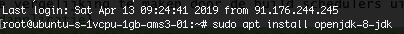
\includegraphics[scale=0.9]{InstallatieJenkins1}
        \caption{Installatie Jenkins, stap 1} \label{InstallatieJenkins1}
    \end{figure}
    
    \begin{figure}	
        \centering
        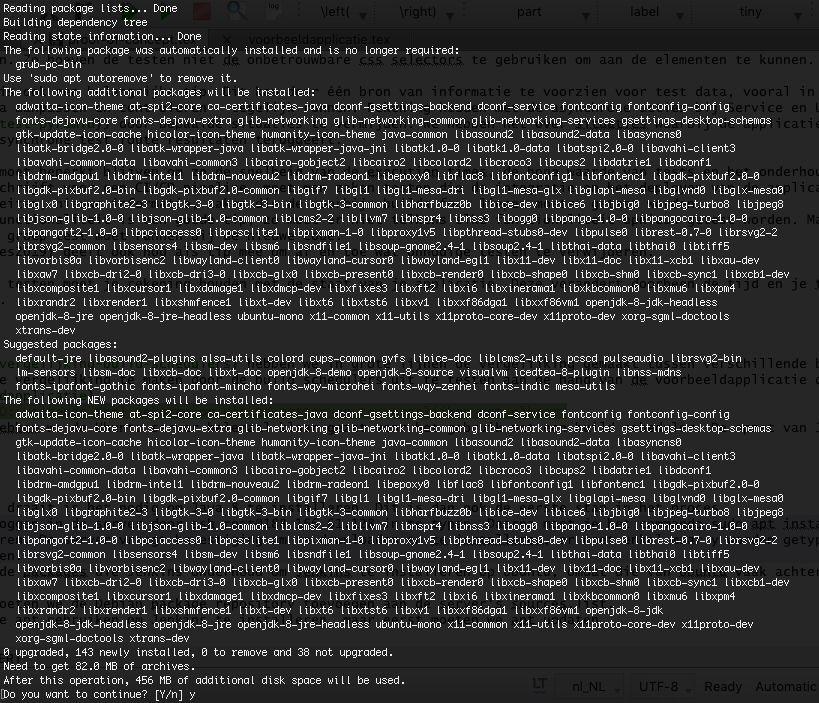
\includegraphics[scale=0.5]{InstallatieJenkins2}
        \caption{Installatie Jenkins, stap 2} \label{InstallatieJenkins2}
    \end{figure}
    
    \begin{figure}	
        \centering
        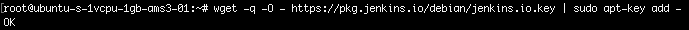
\includegraphics[scale=0.65]{InstallatieJenkins3}
        \caption{Installatie Jenkins, stap 3} \label{InstallatieJenkins3}
    \end{figure}
    
    \begin{figure}	
        \centering
        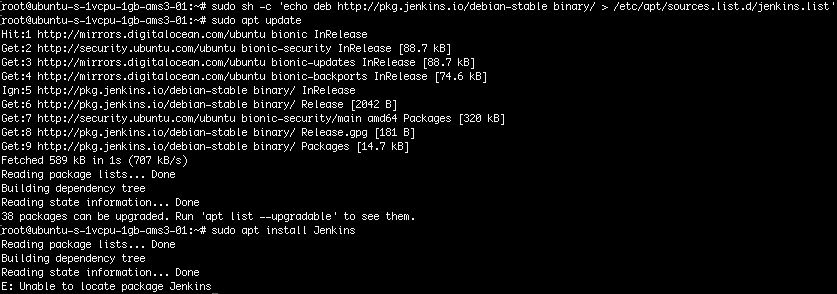
\includegraphics[scale=0.5]{InstallatieJenkins4}
        \caption{Installatie Jenkins, stap 4} \label{InstallatieJenkins4}
    \end{figure}
    
    \begin{figure}	
        \centering
        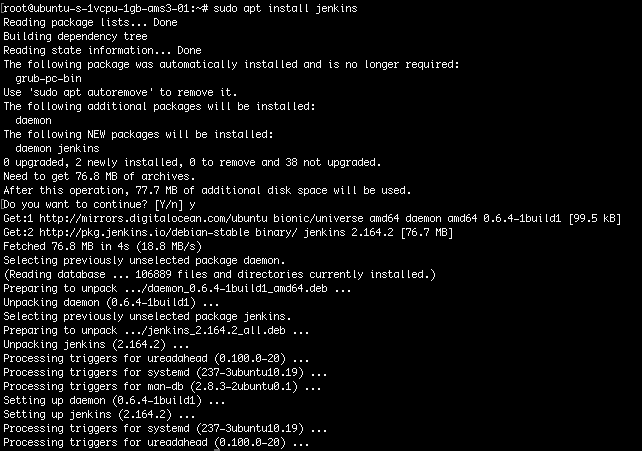
\includegraphics[scale=0.65]{InstallatieJenkins5}
        \caption{Installatie Jenkins, stap 5} \label{InstallatieJenkins5}
    \end{figure}

    
    Na de installatie kunnen we Jenkins starten op de server door het commando 'sudo systemctl start jenkins' in te typen. Omdat dit commando geen uitvoer geeft moeten we het commando 'sudo systemctl status jenkins' intypen. Als je active ziet verschijnen wil dit zeggen dan Jenkins runt op de Ubuntu server. Deze stappen kan je volgen in figuur \ref{Jenkins1}.
    Eens Jenkins gestart is moeten we die kunnen aanspreken vanuit een browser, daarom moeten we de regels van de firewall wat aanpassen. Standaard draait Jenkins op poort 8080. Deze moet geopend worden op de server door het commando 'sudo ufw allow 8080' in te voeren zoals in figuur \ref{Jenkins2} te zien is.
    
    Nu moet Jenkins geconfigureerd worden, dit moet vanuit elke browser gebeuren.
    Er moet naar http://188.166.61.128:8080 gesurft worden om de configuratie te voltooien, zoals aangegeven in figuur \ref{Jenkins3}. De cijfers voor de :8080 staan voor het ip-adres van de Ubuntu server, de :8080 is de poort waar je naartoe wil gaan. Hier draait - zoals in de vorige stappen geconfigureerd - Jenkins op.
    Het paswoord dat gevraagd wordt is terug te vinden in de 'initialAdminPassword' file dat zich in de map '/var/lib/jenkins/secrets/' bevindt op de server. Het is voldoende om op de server volgend commando in te voeren: 'sudo cat /var/lib/jenkins/secrets/initialAdminPassword'. Het paswoord dat als uitvoer komt moet gekopieerd worden en geplakt worden in het invoerveld in de web browser zoals in figuur \ref{Jenkins4} te zien is.
    De volgende stap is het installeren van de voorgestelde plugins. Er wordt gevraagd om een eerste user te configureren, maar voor deze doeleinden is het voldoende om als admin en met het initiële paswoord verder te gaan, er mag dus op 'Continue as admin' gedrukt worden. Nu moet er instantie gemaakt worden door te controleren of de url die ingevuld is klopt met de url die enkele stappen geleden ingegeven is om de webpagina te openen. Wanneer deze klopt kan er op 'Save and Finish' en nadien op 'Start using Jenkins' geklikt worden. Het dashboard van Jenkins wordt geopend. Bovenstaande stappen kan u allemaal volgen in de figuren \ref{Jenkins5}, \ref{Jenkins6}, \ref{Jenkins7}, \ref{Jenkins8}, \ref{Jenkins9} en \ref{Jenkins10}.
    
    \begin{figure}	
        \centering
        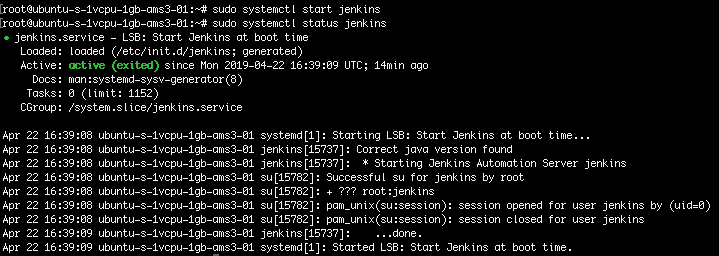
\includegraphics[scale=0.6]{Jenkins1}
        \caption{Opzetten Jenkins, stap 1} \label{Jenkins1}
    \end{figure}
    
    \begin{figure}
        \centering
        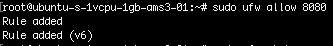
\includegraphics{Jenkins2}
        \caption{Opzetten Jenkins, stap 2} \label{Jenkins2}
    \end{figure}
    
    \begin{figure}	
        \centering
        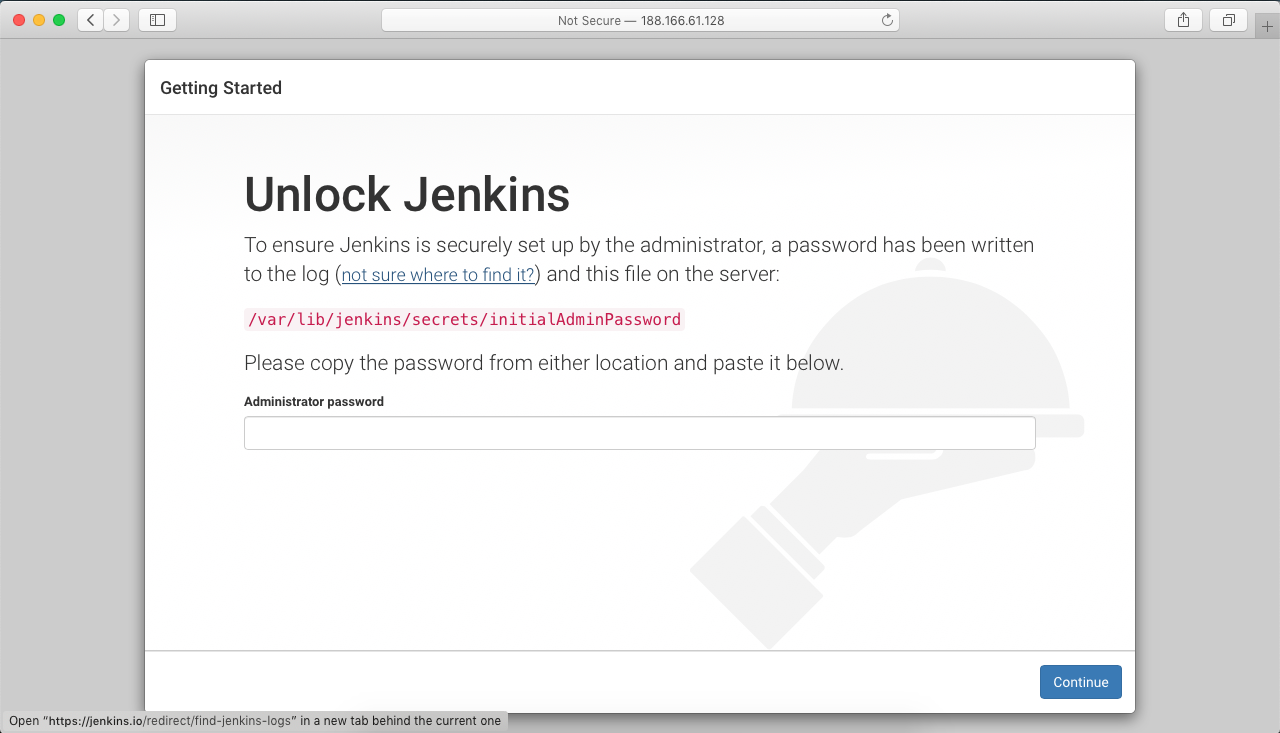
\includegraphics[scale=0.35]{Jenkins3}
        \caption{Opzetten Jenkins, stap 3} \label{Jenkins3}
    \end{figure}
    
    \begin{figure}	
        \centering
        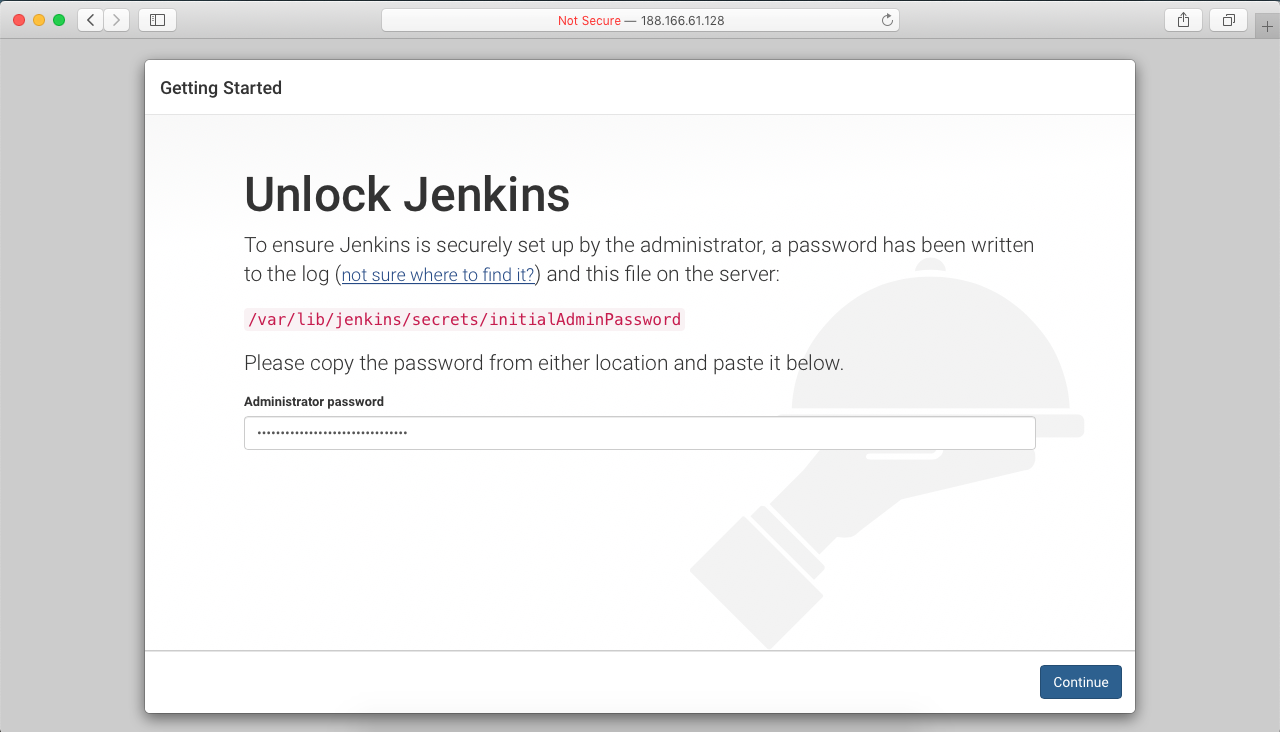
\includegraphics[scale=0.35]{Jenkins4}
        \caption{Opzetten Jenkins, stap 4} \label{Jenkins4}
    \end{figure}
    
    \begin{figure}	
        \centering
        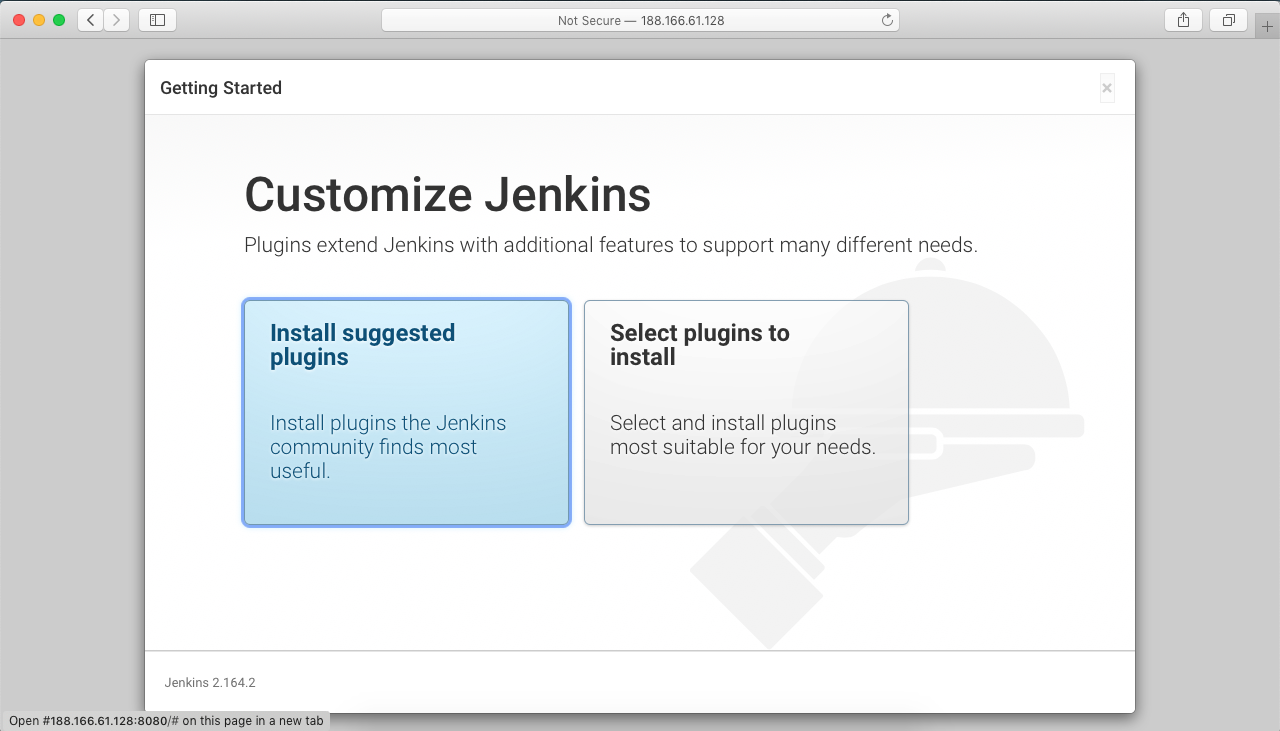
\includegraphics[scale=0.35]{Jenkins5}
        \caption{Opzetten Jenkins, stap 5} \label{Jenkins5}
    \end{figure}
    
    \begin{figure}	
        \centering
        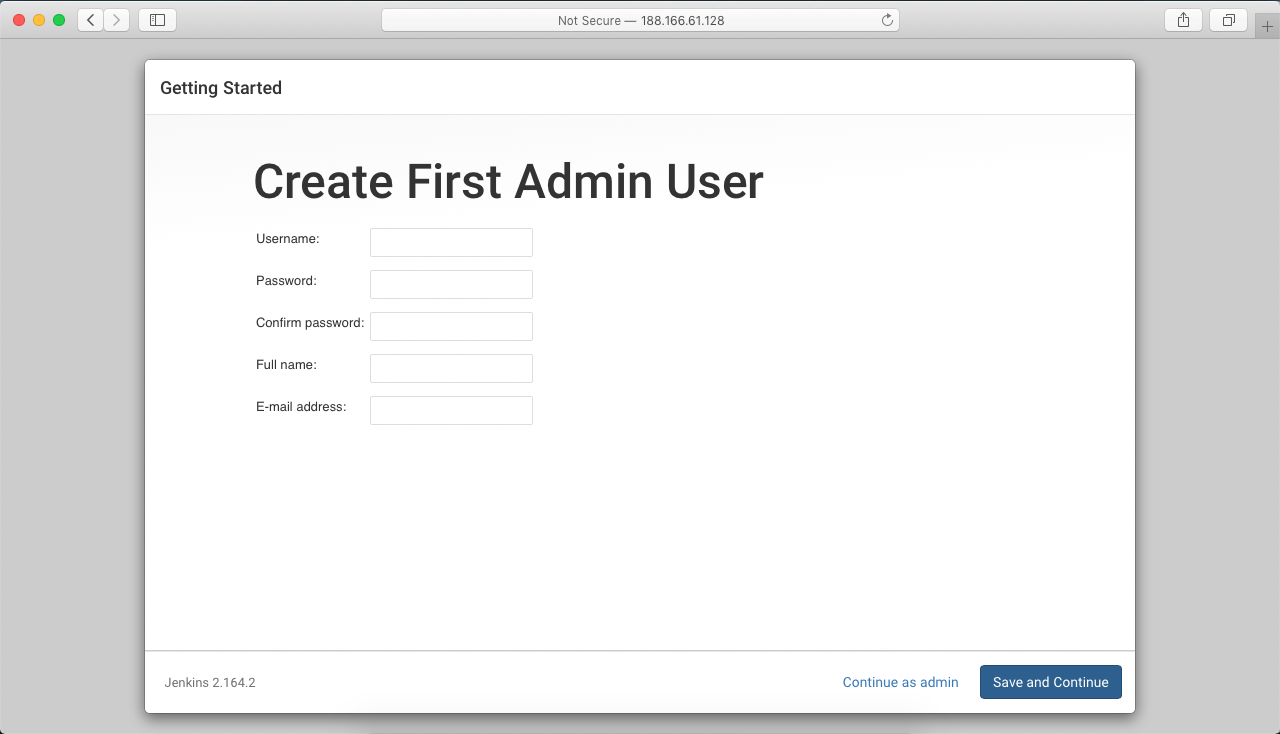
\includegraphics[scale=0.35]{Jenkins6}
        \caption{Opzetten Jenkins, stap 6} \label{Jenkins6}
    \end{figure}

    \begin{figure}	
        \centering
        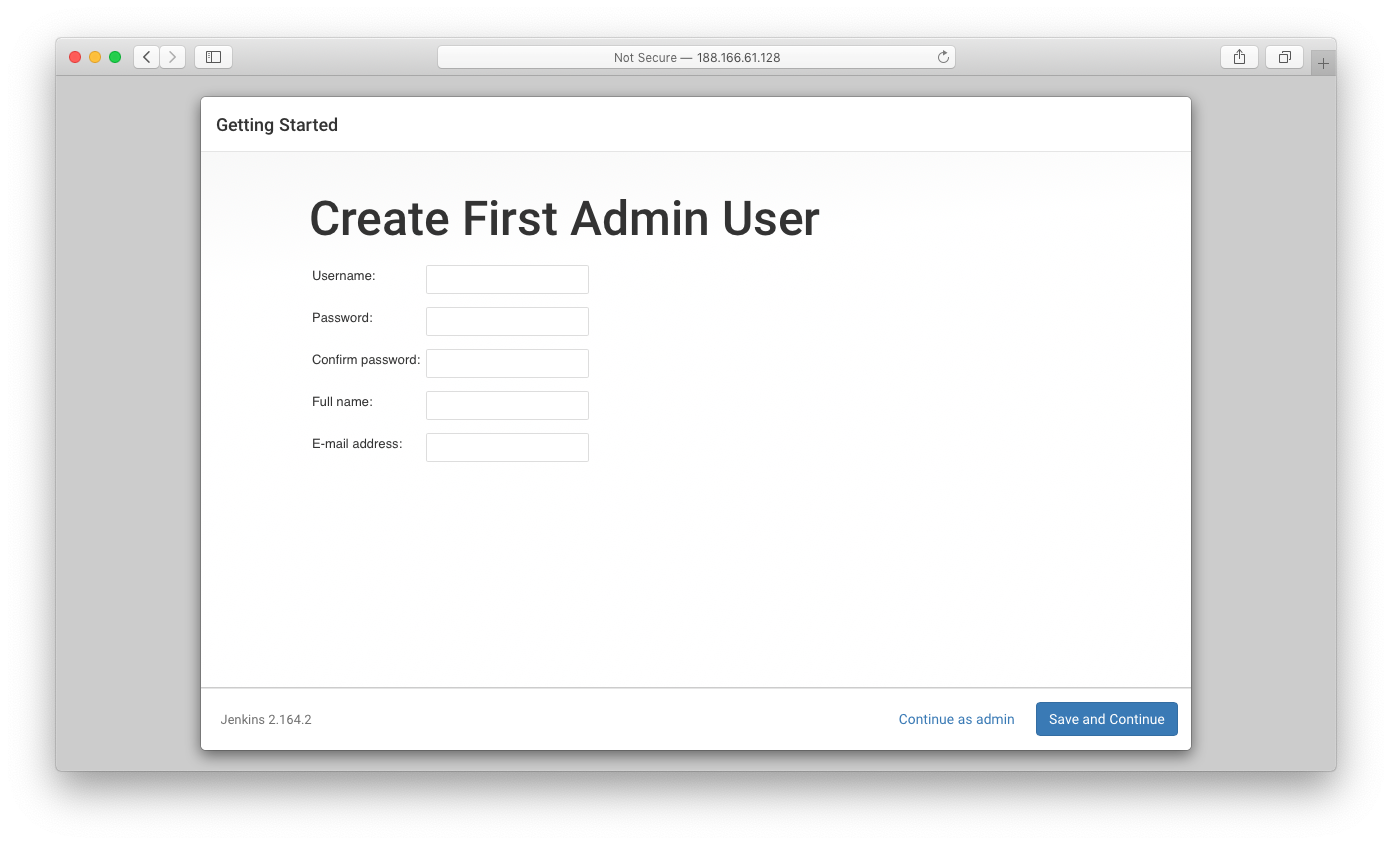
\includegraphics[scale=0.35]{Jenkins7}
        \caption{Opzetten Jenkins, stap 7} \label{Jenkins7}
    \end{figure}
    
    \begin{figure}	
        \centering
        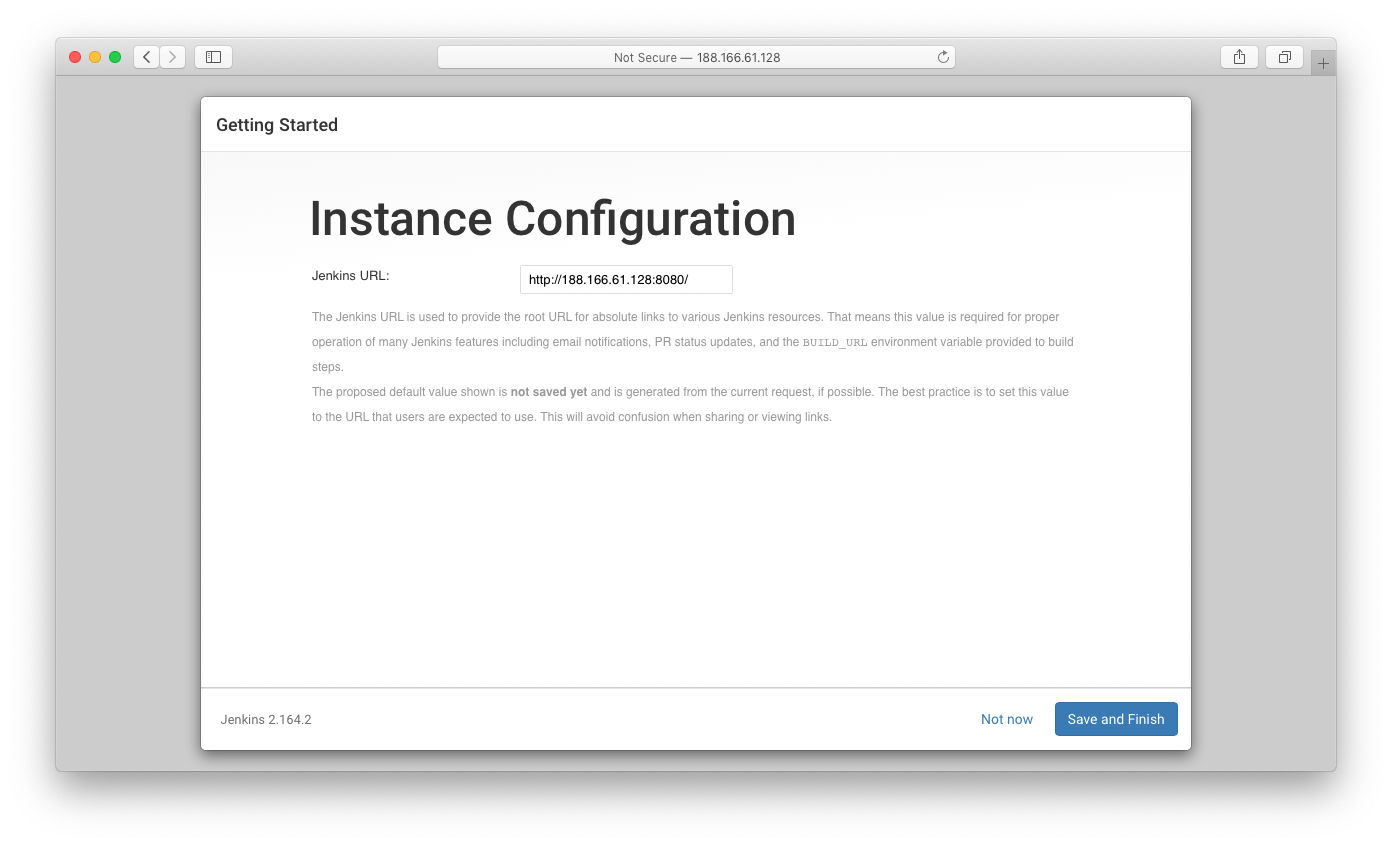
\includegraphics[scale=0.35]{Jenkins8}
        \caption{Opzetten Jenkins, stap 8} \label{Jenkins8}
    \end{figure}
    
    \begin{figure}	
        \centering
        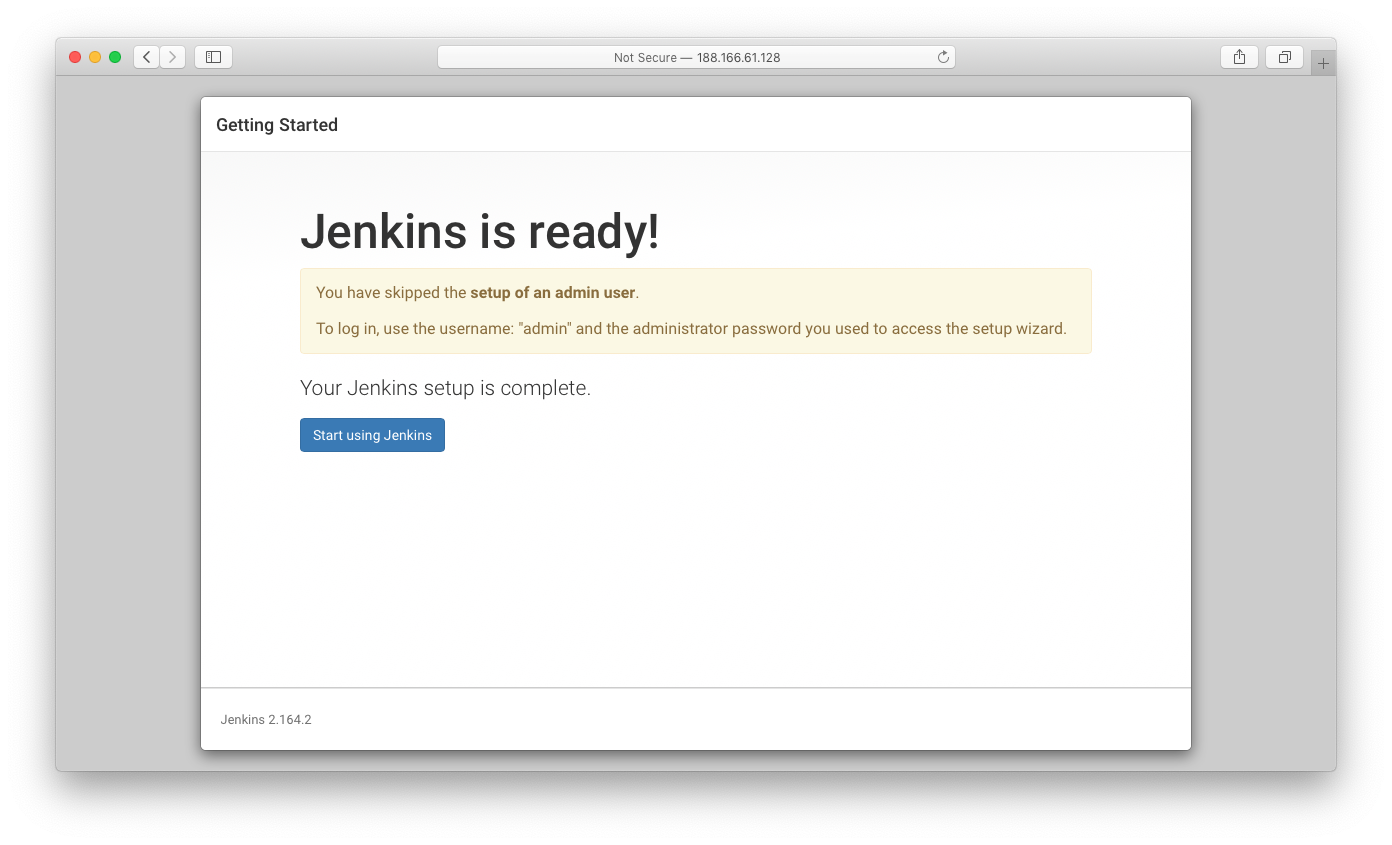
\includegraphics[scale=0.35]{Jenkins9}
        \caption{Opzetten Jenkins, stap 9} \label{Jenkins9}
    \end{figure}
    
    \begin{figure}	
        \centering
        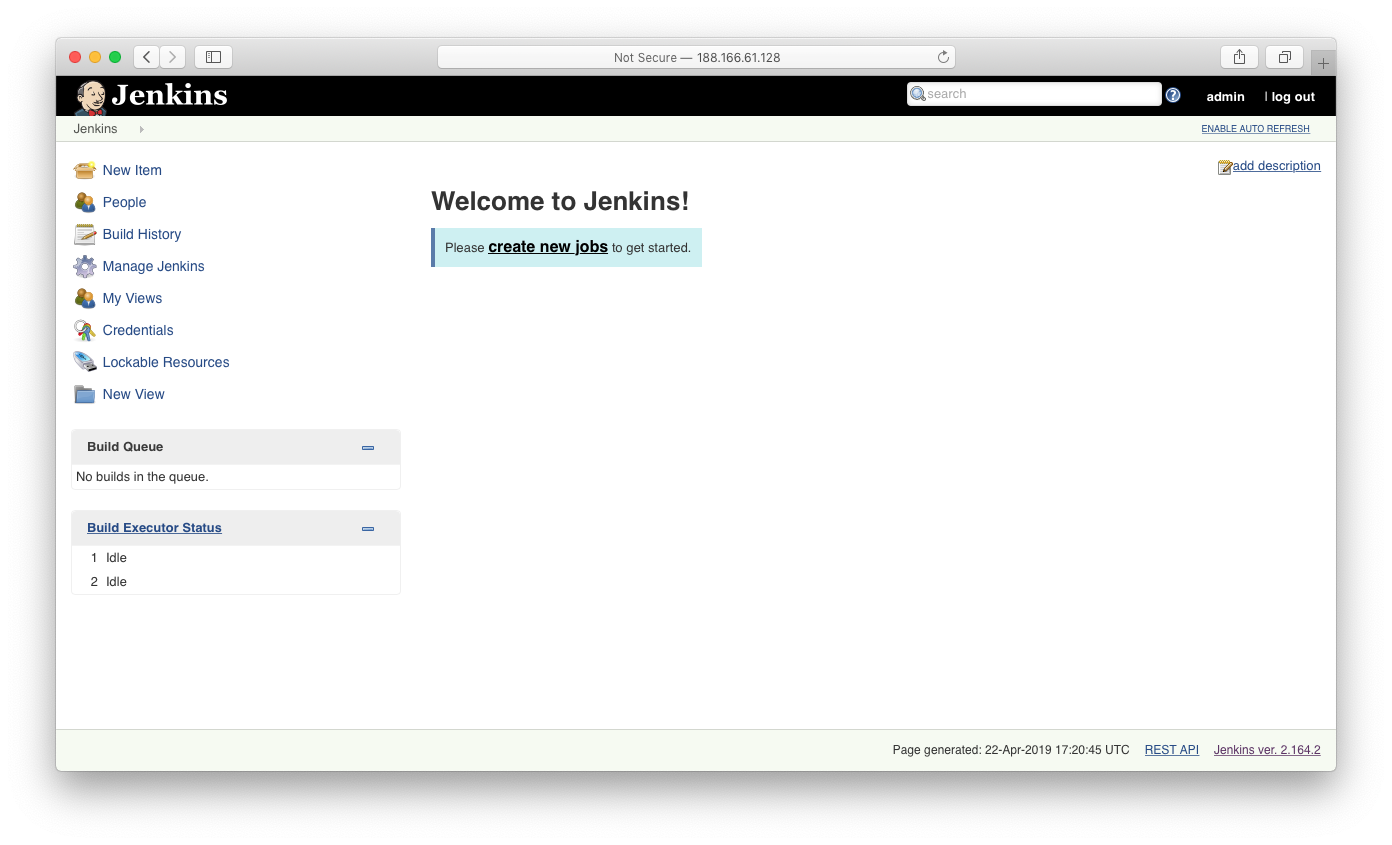
\includegraphics[scale=0.35]{Jenkins10}
        \caption{Opzetten Jenkins, stap 10} \label{Jenkins10}
    \end{figure}
    
    %TODO: https://sap.github.io/jenkins-library/scenarios/ui5-sap-cp/Readme/!!!!!!!!!
    %TODO: https://blogs.sap.com/2017/11/21/continuous-delivery-with-jenkins-pipelines/
    %TODO: http://www.sapspot.com/ci-cd-for-sapui5-on-scp-neo-with-gitlab/
    %TODO: OPA test via Selenium: https://www.agiletrailblazers.com/blog/modernized-technology/automated-testing-with-selenium-grid-and-jenkins-in-3-steps
    
    
\section{Conclusie}
\label{sec:conclusie}


%%=============================================================================
%% Conclusie
%%=============================================================================

\chapter{Conclusie}
\label{ch:conclusie}

% TODO: Trek een duidelijke conclusie, in de vorm van een antwoord op de
% onderzoeksvra(a)g(en). Wat was jouw bijdrage aan het onderzoeksdomein en
% hoe biedt dit meerwaarde aan het vakgebied/doelgroep? 
% Reflecteer kritisch over het resultaat. In Engelse teksten wordt deze sectie
% ``Discussion'' genoemd. Had je deze uitkomst verwacht? Zijn er zaken die nog
% niet duidelijk zijn?
% Heeft het onderzoek geleid tot nieuwe vragen die uitnodigen tot verder 
%onderzoek?

\lipsum[76-80]



%%=============================================================================
%% Bijlagen
%%=============================================================================

\appendix
\renewcommand{\chaptername}{Appendix}

%%---------- Onderzoeksvoorstel -----------------------------------------------

\chapter{Onderzoeksvoorstel}

Het onderwerp van deze bachelorproef is gebaseerd op een onderzoeksvoorstel dat vooraf werd beoordeeld door de promotor. Dat voorstel is opgenomen in deze bijlage.

% Verwijzing naar het bestand met de inhoud van het onderzoeksvoorstel
%---------- Inleiding ---------------------------------------------------------

\section{Introductie} % The \section*{} command stops section numbering
\label{sec:introductie}

Hier introduceer je werk. Je hoeft hier nog niet te technisch te gaan.

Je beschrijft zeker:

\begin{itemize}
  \item de probleemstelling en context
  \item de motivatie en relevantie voor het onderzoek
  \item de doelstelling en onderzoeksvraag/-vragen
\end{itemize}

%---------- Stand van zaken ---------------------------------------------------

\section{State-of-the-art}
\label{sec:state-of-the-art}

Hier beschrijf je de \emph{state-of-the-art} rondom je gekozen onderzoeksdomein. Dit kan bijvoorbeeld een literatuurstudie zijn. Je mag de titel van deze sectie ook aanpassen (literatuurstudie, stand van zaken, enz.). Zijn er al gelijkaardige onderzoeken gevoerd? Wat concluderen ze? Wat is het verschil met jouw onderzoek? Wat is de relevantie met jouw onderzoek?

Verwijs bij elke introductie van een term of bewering over het domein naar de vakliteratuur, bijvoorbeeld~\autocite{Doll1954}! Denk zeker goed na welke werken je refereert en waarom.

% Voor literatuurverwijzingen zijn er twee belangrijke commando's:
% \autocite{KEY} => (Auteur, jaartal) Gebruik dit als de naam van de auteur
%   geen onderdeel is van de zin.
% \textcite{KEY} => Auteur (jaartal)  Gebruik dit als de auteursnaam wel een
%   functie heeft in de zin (bv. ``Uit onderzoek door Doll & Hill (1954) bleek
%   ...'')

Je mag gerust gebruik maken van subsecties in dit onderdeel.

%---------- Methodologie ------------------------------------------------------
\section{Methodologie}
\label{sec:methodologie}

Hier beschrijf je hoe je van plan bent het onderzoek te voeren. Welke onderzoekstechniek ga je toepassen om elk van je onderzoeksvragen te beantwoorden? Gebruik je hiervoor experimenten, vragenlijsten, simulaties? Je beschrijft ook al welke tools je denkt hiervoor te gebruiken of te ontwikkelen.

%---------- Verwachte resultaten ----------------------------------------------
\section{Verwachte resultaten}
\label{sec:verwachte_resultaten}

Hier beschrijf je welke resultaten je verwacht. Als je metingen en simulaties uitvoert, kan je hier al mock-ups maken van de grafieken samen met de verwachte conclusies. Benoem zeker al je assen en de stukken van de grafiek die je gaat gebruiken. Dit zorgt ervoor dat je concreet weet hoe je je data gaat moeten structureren.

%---------- Verwachte conclusies ----------------------------------------------
\section{Verwachte conclusies}
\label{sec:verwachte_conclusies}

Hier beschrijf je wat je verwacht uit je onderzoek, met de motivatie waarom. Het is \textbf{niet} erg indien uit je onderzoek andere resultaten en conclusies vloeien dan dat je hier beschrijft: het is dan juist interessant om te onderzoeken waarom jouw hypothesen niet overeenkomen met de resultaten.



%%---------- Andere bijlagen --------------------------------------------------
% TODO: Voeg hier eventuele andere bijlagen toe
%\input{...}

%%---------- Referentielijst --------------------------------------------------

\printbibliography[heading=bibintoc]

\end{document}
